  %%%%%%%%%%%%%%%%%%%%%%%%%%%%%%%%%%%%%%%%%%%%%%%%%%%%%%%%%%%%%%%%%%%%%%
% LaTeX Example: Project Report

%%% Preamble
\documentclass[paper=a4, fontsize=11pt, abstract=on]{scrartcl}
\usepackage[T1]{fontenc}
\usepackage{fourier}
\usepackage{tabularx}
\usepackage[utf8]{inputenc}
\usepackage{hyperref}





\usepackage{listings}
\usepackage{color}

\definecolor{dkgreen}{rgb}{0,0.6,0}
\definecolor{gray}{rgb}{0.5,0.5,0.5}
\definecolor{mauve}{rgb}{0.58,0,0.82}
\lstset{frame=tb,
  language=[Visual]C++,
  aboveskip=3mm,
  belowskip=3mm,
  showstringspaces=false,
  columns=flexible,
  basicstyle={\small\ttfamily},
  numbers=none,
  numberstyle=\tiny\color{gray},
  keywordstyle=\color{blue},
  commentstyle=\color{dkgreen},
  stringstyle=\color{mauve},
  breaklines=true,
  breakatwhitespace=true,
  tabsize=3
}
\usepackage{graphicx}
\usepackage{caption}
\usepackage{subcaption}

\usepackage[english]{babel}															% English language/hyphenation
\usepackage[protrusion=true,expansion=true]{microtype}	
\usepackage{amsmath,amsfonts,amsthm} % Math packages

\usepackage{url}
%\usepackage[hang, small,labelfont=bf,up,textfont=it,up]{caption}


%%% Custom sectioning
\usepackage{sectsty}
\allsectionsfont{\normalfont\scshape}
\usepackage{float}
\usepackage{amsmath}
\usepackage{mathtools}
\usepackage{ragged2e}

\usepackage{nomencl}
\makenomenclature

%%% Custom headers/footers (fancyhdr package)
\usepackage{fancyhdr}
\pagestyle{fancyplain}
\fancyhead{}											% No page header
\fancyfoot[L]{}											% Empty 
\fancyfoot[C]{}											% Empty
\fancyfoot[R]{\thepage}									% Pagenumbering
\renewcommand{\headrulewidth}{0pt}			% Remove header underlines
\renewcommand{\footrulewidth}{0pt}				% Remove footer underlines
\setlength{\headheight}{13.6pt}
   \renewcommand*\abstractname{Summary}

%%% Equation and float numbering
\numberwithin{equation}{section}		% Equationnumbering: section.eq#
\numberwithin{figure}{section}			% Figurenumbering: section.fig#
\numberwithin{table}{section}				% Tablenumbering: section.tab#


%%% Maketitle metadata

\newcommand{\horrule}[1]{\rule{\linewidth}{#1}} 	% Horizontal rule

\title{
		%\vspace{-1in} 	
		\usefont{OT1}{bch}{b}{n}
		\normalfont \normalsize \textsc{} \\ [25pt]
		
\includegraphics[width=0.3\linewidth]{ubc.png} \\
		%
\includegraphics[width=0.4\linewidth]{tru}		
		\horrule{0.5pt} \\[0.2cm]
		\huge Programming Assignment \#3 : Solving Incompressible Energy Equation  \\
		\horrule{2pt} \\[0.005cm]
}
\author{
		\normalfont 								\normalsize
        Jerin Roberts\\[-5pt]		\normalsize
        \today
}
\date{}




%%% Begin document
\begin{document}
\maketitle
\begin{center}
\begin{tabular}{l r}


Supervisor: & Dr. Carl Ollivier-Gooch  \\ % supervisor
Locations: & University of British Columbia


\end{tabular}
\end{center}



\newpage
\tableofcontents
\listoffigures
\listoftables
\newpage
\lstset{language=[Visual]C++}
\section{Introduction}



 The are many physical phenomenons in physics and engineering that require linear and non-linear partial differential equations to described the true nature of the system. Solving these systems analytically and finding exact solutions for these equations can be difficult and often require simplifications that ultimately don't fully represent the problem being investigated. Numerical methods for solving PDE's provides a means for finding approximations to the exact solutions without having to make sacrificial simplifications. With recent advancements in computational technology numerical methods can now be easily applied to large and difficult problems that would otherwise be impossible to solve. 
\subsection{Problem Overview}
Numerical problems are essentially solved by breaking the entire solution domain into small discrete points (mesh) and finding the solution at or around these areas. Each point requires the solving the differential equations that represent physical phenomenon being investigated. Since the exact solution cannot be computed, it is instead approximated using various techniques and methods. In this assignment the 2D in-compressible laminar energy equation is applied to a rectangular channel for a given velocity field. The problem will employ an second ordered centered flux calculation with both implicit and explicit euler timer advance methods. The implicit method will be solved using approximate factorization and Gauss-Jordan elimination via the Thomas algorithm. Boundary conditions will be implement using ghost cells allowing the interior scheme to remain the same during calculation of bordering cells. The ghost cells are calculated such the boundary condition is enforced at $i=1/2$.



\section{Implementation}
\subsection{Program Overview}
The C/C++language was selected for this programming assignment. The scripts were compiled using g++/gcc version 5.4.0 on Ubuntu 16.04.02 and are available in the attached zip or for clone via the link provided: \url{https://github.com/j16out/cfd510} . The program itself is broken into 3 pieces and two levels to produce a modular set that makes it easier to apply to different problems. The highest level contains the "macro" or the main function which can be modified for different problems. 
The numerical directory contains numerical.cpp script and its header file numerical.hpp. This set contains all the functions necessary for solving the problem numerically. The appendix contains the .hpp file which lists all functions with a short description of each. The vroot directory contains the scripts necessary for drawing data. These scripts make use of the ROOT-v6 libraries. ROOT is a popular data analysis framework primarily written in C++ and Phython. For more information on ROOT libraries visit the link provided: \url{https://root.cern.ch/} .
The functions act on a structure called $carray$ which contains the solution domain array and its various parameters. The struct contains the main array, its defined working area (mesh size), data storage vectors, iteration count, and the represented dimension between points. Having these organized in a struct provides a compact way of passing and modifying the array and all its pertinent parameters. The outline of the struct used for the energy equation problem is shown below.

 

\begin{lstlisting}
struct carray{
//arrays
double f1 [maxx][maxy];//flux or temp space
double T1 [maxx][maxy];//Temperature
double v1 [maxx][maxy];//x velocity
double u1 [maxx][maxy];//y velocity
//array attributes
int sizex = maxx;
int sizey = maxy;
double DIMx = 0.0;
double DIMy = 0.0;
//time
double ctime = 0;
};
\end{lstlisting}
 
\subsection{Flux Calculation}


 The program was built and tested in small components to ensure its correctness. The flux integral without the source term was run and compared to the exact solution for the flux integral as displayed in equation \ref{eflux}. This exact integral can be approximated by a scheme of cell volume averages as shown in equation \ref{xflux} for x and \ref{yflux}. The problem will employ a second ordered centered flux calculation which is found on the RHS of the discretized energy equation.


\begin{equation}
\label{eflux}
\iint \Bigg(u\frac{\partial T}{\partial xt} + v\frac{\partial T}{\partial y}-\frac{\bigtriangledown^2T}{Re Pr}\Bigg)dA
\end{equation}



  \begin{equation}
\label{xflux}
\frac{-1}{\triangle x}\Bigg(\frac{u_{i+1,j}\overline{T}_{i+1,j}^n-u_{i-1,j}\overline{T}_{i-1,j}^n}{2}-\frac{1}{Re Pr}\Bigg(\frac{\overline{T}_{i+1,j}^n-2\overline{T}_{i,j}^n+\overline{T}_{i-1,j}^n}{2\triangle x}\Bigg)\Bigg)
\end{equation}

 \begin{equation}
\label{yflux}
 \frac{1}{\triangle y}\Bigg(\frac{v_{i,j+1}\overline{T}_{i,j+1}^n-u_{i,j-1}\overline{T}_{i,j-1}^n}{2}-\frac{1}{Re Pr}\Bigg(\frac{\overline{T}_{i,j+1}^n-2\overline{T}_{i,j}^n+\overline{T}_{i,j-1}^n}{2\triangle y}\Bigg)\Bigg)
\end{equation}

The flux was calculated using the function $compute\_ flux()$, which is shown below. The function calls two other functions which grab the necessary data using the $surr$ struct from the current solution. The flux calculated using $calc\_ newcell()$ is then stored on the $carray$ struct under the $f1$ array.

\begin{lstlisting}
void compute_Flux(carray & myarray)
{
surr mysurr;
for(int j = 1; j < myarray.sizey-1; ++j)
{
    for(int i = 1; i < myarray.sizex-1; ++i)
    {
    //----get surrounding cells and compute new cell----//
    get_nsurcells(myarray, i, j, mysurr);
    //-----update current cell----//
    double newcell = calc_newcell(myarray, mysurr);    
    myarray.f1[i][j] = newcell;   
    }
}
}
\end{lstlisting}



\begin{table}[H]
\begin{center}
    \begin{tabular}{ | p{0.13\linewidth} | p{0.2\linewidth} |p{0.1\linewidth} |p{0.1\linewidth} |p{0.1\linewidth} |}
 \hline  
     \RaggedRight \textbf{Mesh Size}
    &\RaggedRight \textbf{$L^2$norm}
    &\RaggedRight \textbf{$\triangle x$}
    &\RaggedRight \textbf{Order}
    \\ \hline  
           \RaggedRight 10 x 10
    &\RaggedRight 8.773$*10^{-1}$
    &\RaggedRight 0.1
    &\RaggedRight -
    \\ \hline 
    \RaggedRight 20 x 20
    &\RaggedRight 2.230 $*10^{-1}$
    &\RaggedRight 0.05
    &\RaggedRight 1.981
    \\ \hline 
           \RaggedRight 40 x 40
    &\RaggedRight 9.942 $*10^{-2}$
    &\RaggedRight 0.025
    &\RaggedRight 1.986
    \\ \hline 
           \RaggedRight 80 x 80
    &\RaggedRight 1.401$*10^{-2}$
    &\RaggedRight 0.0125
    &\RaggedRight 1.991
    \\ \hline       
   \end{tabular}
\end{center} 
\caption{Table of $L^2$ norms for increasing mesh size of flux integral}
\label{norm1} 
\end{table}

The correctness of the flux integral was validated using the exact computer flux. The $L_2$ norms for the flux calculation are displayed in table \ref{norm1}. The order of accuracy for the scheme was determined using the log log method as displayed in figure \ref{ord}. The order of accuracy for this scheme was estimated to be 2nd order accurate based on the $L_2$ data from 8 different meshes.     
    
  

\begin{figure}[H]
\centering
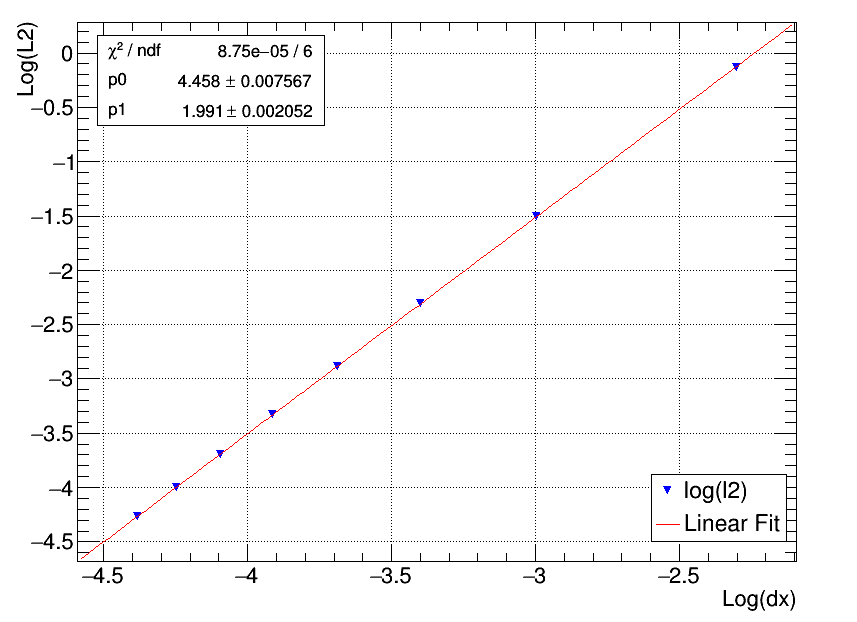
\includegraphics[width=0.75\linewidth]{order}
\caption{Calculated Order of Accuracy without source}
\label{ord}
\end{figure}


This matches what was expect by implementing a 2nd order interior flux evaluation and boundary schemes. It should be noted as seen in figure \ref{qq22} the relative error decreases when refining the mesh. This is expect as the numerical solution is a discrete representation of the continuous exact solution. 

 




\subsection{Source Term Validation}
An exact solution for the source term exists and was used to validate the correctness of the computed source term. The same procedure as described above was used to find the $L_2$ norms for the source term and the complete flux integral (figure \ref{fs} and table \ref{tfs}). The entire calculation is done in the subroutine $calc\_ newcell()$ which is displayed below.
\begin{lstlisting}
double calc_newcell(carray & myarray, surr & s1){
double chx = myarray.DIMx;
double chy = myarray.DIMy;
//flux integral
double a = (s1.uip1_j * s1.Tip1_j  -  s1.uim1_j * s1.Tim1_j)/(2.0);
double b = (s1.Tip1_j  - 2.0*s1.Ti_j + s1.Tim1_j)/(chx*(RE*PR));
double c = (s1.vi_jp1 * s1.Ti_jp1  -  s1.vi_jm1 * s1.Ti_jm1)/(2.0);
double d = (s1.Ti_jp1  - 2.0*s1.Ti_j + s1.Ti_jm1)/(chy*(RE*PR));
//source term
double e = (2.0*pow((s1.uip1_j-s1.uim1_j)/(2.0*chx),2)+2.0*pow((s1.vi_jp1-s1.vi_jm1)/(2.0*chy),2));
double f = pow(((s1.vip1_j-s1.vim1_j)/(2.0*chx))+((s1.ui_jp1-s1.ui_jm1)/(2.0*chy)), 2);
double source = (EC/RE)*(e+f);
//add altogether
double newcell = 1.0*((-1.0/chx)*(a-b)   +   (-1.0/chy)*(c-d))   +   source;
return newcell;
}
\end{lstlisting}




 \begin{table}[H]
\begin{center}
    \begin{tabular}{ | p{0.13\linewidth} | p{0.2\linewidth} |p{0.1\linewidth} |p{0.1\linewidth} |p{0.1\linewidth} |}
 \hline  
     \RaggedRight \textbf{Mesh Size}
    &\RaggedRight \textbf{$L^2$norm}
    &\RaggedRight \textbf{$\triangle x$}
    &\RaggedRight \textbf{Order}
    \\ \hline  
           \RaggedRight 10 x 10
    &\RaggedRight 8.796$*10^{-2}$
    &\RaggedRight 0.1
    &\RaggedRight -
    \\ \hline 
    \RaggedRight 20 x 20
    &\RaggedRight 2.235 $*10^{-2}$
    &\RaggedRight 0.05
    &\RaggedRight 1.981
    \\ \hline 
           \RaggedRight 40 x 40
    &\RaggedRight 5.613 $*10^{-3}$
    &\RaggedRight 0.025
    &\RaggedRight 1.985
    \\ \hline 
           \RaggedRight 80 x 80
    &\RaggedRight 1.405$*10^{-3}$
    &\RaggedRight 0.0125
    &\RaggedRight 1.991
    \\ \hline 

    \end{tabular}
\end{center} 
\caption{Table of $L^2$ norms for increasing mesh size of flux integral with source}
\label{tfs} 
\end{table}



\begin{figure}[H]
\centering
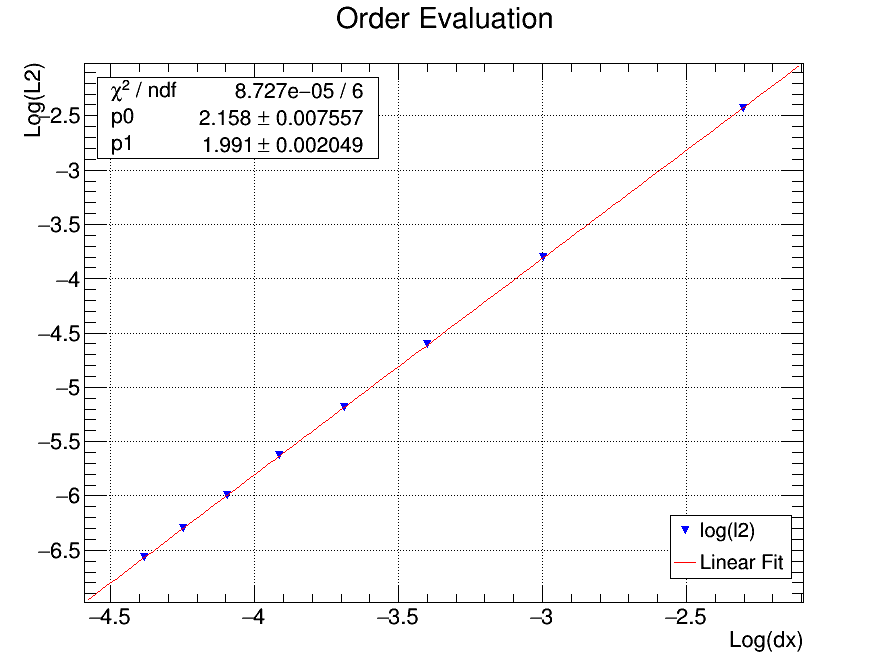
\includegraphics[width=0.7\linewidth]{orderws}
\caption{Calculated Order of Accuracy with of flux integral with source}
\label{fs}
\end{figure}



Once the flux integral had been validated and its correctness confirmed two methods were coded for time advance.

\subsection{Explicit Time scheme}



 \begin{equation}
\label{EE}
w^{n+1}=w^n+\triangle t(\lambda w^n)
\end{equation} 

An explicit Euler (EE) time advance scheme was selected and implemented using the $solve\_ arrayEE()$. The method uses current data to advance the solution to the next time level. The expression for Explicit Euler is displayed in equation \ref{EE}. A loop using a given cfl and final time iterates through acquiring the flux and time step calculates the solution of the next time level. The loop is displayed below which also checks for the maximum change in solution to signal when convergence is reached.



\begin{lstlisting}
void time_advance_EE(carray & myarray, double tstep, double & mdiff)
{
mdiff = -1.0;
for(int j = 1; j < myarray.sizey-1; ++j)
{
    for(int i = 1; i < myarray.sizex-1; ++i)
    {  
    double temp = tstep*(myarray.f1[i][j]); 
    if(abs(temp)> mdiff)
    mdiff = abs(temp);      
    myarray.T1[i][j] = myarray.T1[i][j] + temp;
    }
}
}
\end{lstlisting}


The explicit scheme is setup to run find a solution for a 5x1 channel with an intial temperature distribution of $T(x,y,0) = y$. A fully developed fixed temperature distribution is used as the inflow boundary (equation \ref{exEE}) while the outflow boundary is considered fully developed.  The upper wall is held at $T=1$ while the lower at $T=0$. The steady velocity profile $u$ in x direction is given by equation \ref{init} while $v$ is set as zero for all y components.

 
  \begin{equation}
\label{exEE}
T(0,y,t)=y+\frac{3}{4} Pr Ec \bar{u}^2 \bigg(1-(1-2y)^4\bigg)
\end{equation} 
 
 \begin{equation}
\label{init}
u(x,y) = 6\bar{u} y(1-y)
\end{equation} 

The boundary conditions for both the implicit and explicit methods are enforced using the subroutine $set\_ ghostcells()$ as displayed below.
\begin{lstlisting}
void set_ghostcells(carray & myarray)
{
double DIMx = myarray.DIMx;
double DIMy = myarray.DIMy;
double dx = 0.0;
double dy = 0.0;
    //set ghost cells top/bottom
	for(int i = 0; i < myarray.sizex; ++i)
	{
	dx = (i-0.5)*DIMx;
	myarray.T1[i][0] = 3.0*(0.0) - (5.0/2.0)*myarray.T1[i][1] 
	+ (1.0/2.0)*myarray.T1[i][2];	

	myarray.T1[i][myarray.sizey-1] = 3.0*(1.0)- (5.0/2.0)
    *myarray.T1[i][myarray.sizey-2] + (1.0/2.0)*myarray.T1[i][myarray.sizey-3];
	}		
    //set ghost cells inflow/outflow	
	for(int j = 0; j < myarray.sizey; ++j)
	{ 
    dy = (j-0.5)*DIMy;    
	myarray.T1[0][j] = 2.0*( dy+((3.0/4.0)*PR*EC*(pow(U0,2))
	*(1.0-pow((1.0-2.0*dy),4))) ) - myarray.T1[1][j];	
	myarray.T1[myarray.sizex-1][j] = myarray.T1[myarray.sizex-2][j];
	}
}
\end{lstlisting}




The steady state solution will essentially be a linear projection of the inflow boundary, therefore the exact solution can be used to find the error and order of the explicit method. Table \ref{expt} displays the $L2$ norm and the order for varying mesh sizes. Figure \ref{expord} displays the order calculated for explicit euler time advance using the boundaries and initial conditions presented above.

 \begin{table}[H]
\begin{center}
    \begin{tabular}{ | p{0.13\linewidth} | p{0.2\linewidth} |p{0.1\linewidth} |p{0.1\linewidth} |p{0.1\linewidth} | p{0.1\linewidth} |}
 \hline  
     \RaggedRight \textbf{Mesh Size}
    &\RaggedRight \textbf{$L^2$norm}
    &\RaggedRight \textbf{$\triangle x$}
    &\RaggedRight \textbf{$\triangle t$}
    &\RaggedRight \textbf{Order}    
    \\ \hline  
           \RaggedRight 25 x 10
    &\RaggedRight 5.11$*10^{-3}$
    &\RaggedRight 0.2
    &\RaggedRight 0.01
    &\RaggedRight -  
    \\ \hline 
    		\RaggedRight 50 x 20
    &\RaggedRight 1.19 $*10^{-3}$
    &\RaggedRight 0.1
     &\RaggedRight 0.005
    &\RaggedRight 1.855  
    \\ \hline 
           \RaggedRight 100 x 40
    &\RaggedRight  3.46  $*10^{-4}$
    &\RaggedRight 0.05
    &\RaggedRight 0.0025
    &\RaggedRight 1.845   
    \\ \hline 
           \RaggedRight 200 x 80
    &\RaggedRight 9.97$*10^{-5}$
    &\RaggedRight 0.025
    &\RaggedRight 0.00125
    &\RaggedRight 1.844  
    \\ \hline 
 
    \end{tabular}
\end{center} 
\caption{Table of $L^2$ norms for increasing mesh size of explicit method}
\label{expt} 
\end{table}


\begin{figure}[H]
\centering
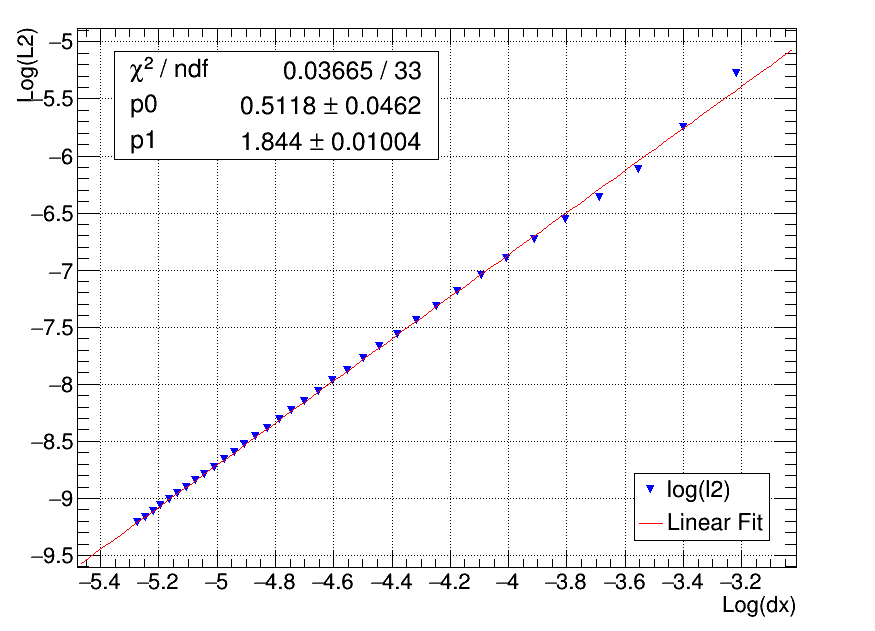
\includegraphics[width=0.85\linewidth]{orderexplicit}
\caption{Calculated Order of Accuracy using explicit method for varying mesh sizes}
\label{expord}
\end{figure}

\subsection{Implicit method}
An implicit euler (IE) time advance scheme was implemented using approximate factorization and a thomas algorithm. One can solve using IE by calling the subroutine $solve\_ array\_ IE()$. The subroutine uses a function called $solve\_ Linsys()$ which moves first row by row then column by column employing approximate factorization to create a system of linear equations in which the cells values within the row are coupled to their neighbors. These tri-diagonal matrix representations of the row/col can be solved using Gauss-Jordan elimination. Using the Thomas algorithm, which is Gauss elimination and back substitution specialized for a tri-diagonal matrix, the subroutine $solve\_ thomas()$ solves a system of the form Ax = b. On the left hand side (LHS) The matrix A can be rewritten into a 2D array with three columns from the three non-zero diagonals. When Vector b is provided as a 1D array (RHS) the subroutine can solve for vectors x. The program uses these tools to calculate the change in solution as shown below.

\begin{lstlisting}
void solve_LinSys(carray & myarray, double tstep, double & mdiff)
{
mdiff = -1.0;
//--linear system num 1---//
crow myrow;
for(int j = 0; j < myarray.sizey; ++j)
{
load_row(myarray, myrow, j, tstep);
solve_thomas(myrow, myarray.sizex);

    for(int i = 0; i < myarray.sizex; ++i)
    {
    myarray.f1[i][j] = myrow.RHS[i];
    }
}
//--linear system num 2---//
ccol mycol;
for(int i = 0; i < myarray.sizex; ++i)
{
load_col(myarray, mycol, i, tstep);
solve_thomas(mycol, myarray.sizey);

    for(int j = 0; j < myarray.sizey; ++j)
    {
    double temp = mycol.RHS[j];
    if(abs(temp) > mdiff)
    mdiff = abs(temp);
    myarray.f1[i][j] = temp;
    myarray.T1[i][j] = temp + myarray.T1[i][j];
    }
}
}
\end{lstlisting}


The structures $crow$ and $ccol$ are the framework for containing the information from the tri-diagonal matrices generated during approximate factorization. The are passed to a function ($load\_ row()$ and $load\_ col()$) which loads them with the correct data to be handed off the the Thomas algorithm for solving. The data for the first step of the algorithm is provided in the Appendix. The implicit scheme was applied to the same problem described for explicit scheme. The implicit was compared to the exact solution for varying meshes. Its order and $L_2$ error are displayed in table \ref{imnorm} and figure \ref{imord}.




 \begin{table}[H]
\begin{center}
    \begin{tabular}{ | p{0.13\linewidth} | p{0.2\linewidth} |p{0.1\linewidth} |p{0.1\linewidth} |p{0.1\linewidth} |}
 \hline  
     \RaggedRight \textbf{Mesh Size}
    &\RaggedRight \textbf{$L^2$norm}
    &\RaggedRight \textbf{$\triangle x$}
    &\RaggedRight \textbf{Order}
    \\ \hline  
           \RaggedRight 25 x 10
    &\RaggedRight 3.48$*10^{-3}$
    &\RaggedRight 0.2
    &\RaggedRight -
    \\ \hline 
    		\RaggedRight 50 x 20
    &\RaggedRight 1.19 $*10^{-3}$
    &\RaggedRight 0.1
    &\RaggedRight 1.761
    \\ \hline 
           \RaggedRight 100 x 40
    &\RaggedRight  3.44  $*10^{-4}$
    &\RaggedRight 0.05
    &\RaggedRight 1.775
    \\ \hline 
           \RaggedRight 200 x 80
    &\RaggedRight 9.97$*10^{-5}$
    &\RaggedRight 0.025
    &\RaggedRight 1.787
    \\ \hline 

    \end{tabular}
\end{center} 
\caption{Table of $L^2$ norms for increasing mesh size of implicit method}
\label{imnorm} 
\end{table}

\begin{figure}[H]
\centering
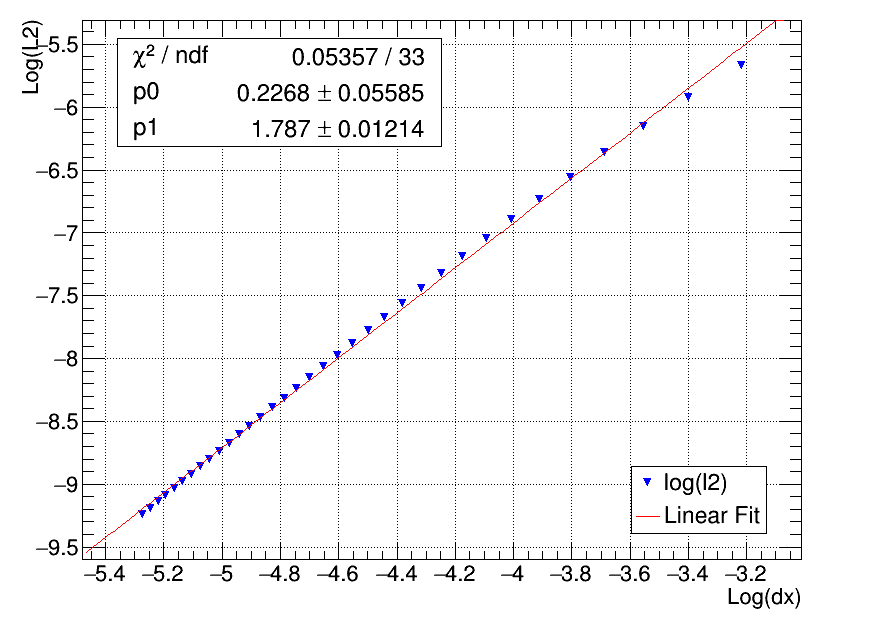
\includegraphics[width=0.75\linewidth]{orderimp}
\caption{Calculated Order of Accuracy using implicit method for varying mesh sizes}
\label{imord}
\end{figure}

\subsection{Efficiency}
The implicit and explicit schemes were timed to compare their relative computing times. Figure \ref{eff} displays the time required for convergence vs the array size. The explicit scheme was run with a $cfl=0.12$ with its maximum stable time step occurring for $cfl=0.145$. 

\begin{figure}[H]
\centering
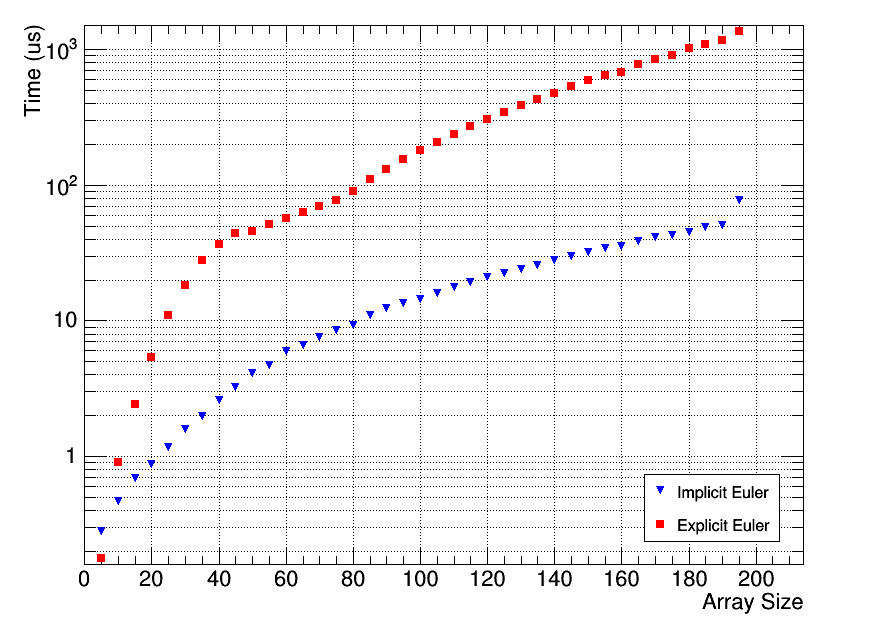
\includegraphics[width=0.75\linewidth]{eff}
\caption{Displays the efficiency trends for both Implicit and explicit Euler for varying mesh sizes}
\label{eff}
\end{figure}

The time step for the implicit scheme was set at $\triangle t = 0.1$. The implicit scheme has high stability for all time steps. However it was found for large time steps that were bigger than the average convergence time, the scheme would need an extra step to converge on steady state properly.

\section{Final Problem}


For the main problem the energy equation was applied to a channel with the conditions from the implicit and explicit tests. For this case two changes are made; The Eckert value is set at a more realistic value of 0.001, and the top wall is now given by $T(x,1,t) = 2-cos(\pi(x-1))$ for $1\leq x \leq 3$ and for everywhere else is $T=1$. The goal was to determine the temperature gradient at the bottom wall. Figure \ref{chan3} displays the steady solution for this channel. A subroutine was used to evaluate the gradient at the wall as a function of x by linearly fitting test points near the boundary. Figure \ref{chan2} displays T gradient as a function of wall length x. The channel was extended beyond 5.0 to  find the maximum gradient along the wall.

\begin{figure}[H]
\centering
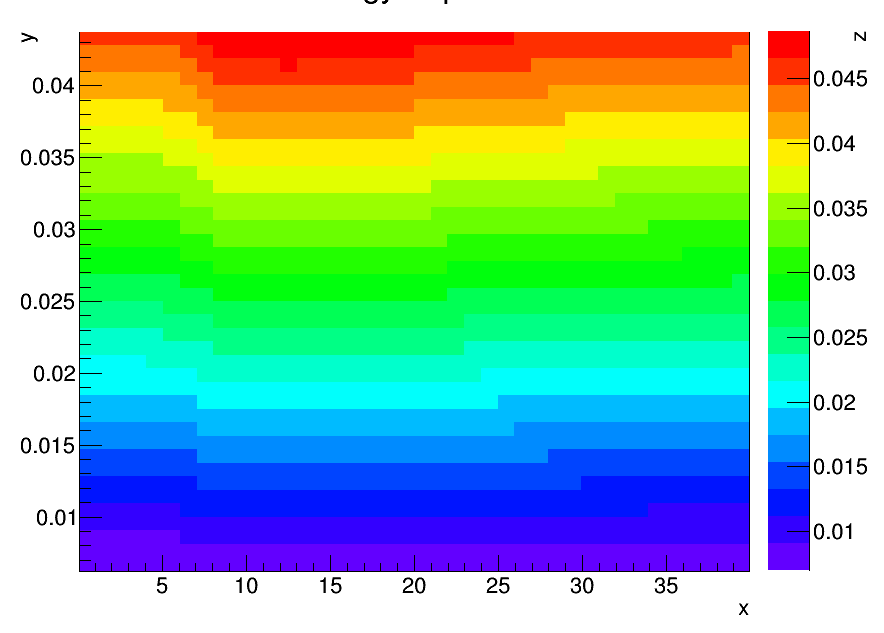
\includegraphics[width=0.75\linewidth]{chan3}
\caption{Displays the solution for temperature in channel}
\label{chan3}
\end{figure}

\subsection{Results}

The solution to the energy problem was computed using implicit euler with$\triangle t=0.1$ and is displayed in figure \ref{chan1}. This data was used to estimate the value for ${dT}/{dy}$ at all points along x. The value of ${dT}/{dy}$ was estimated using a linear fit of for 4 control volumes off the boundary. The solutions for ${dT}/{dy}$ are tabulated in table \ref{chan1} and in \ref{chan2} for increasing grid size. 
\begin{table}[H]
\begin{center}
    \begin{tabular}{ | p{0.2\linewidth} | p{0.2\linewidth} |}
 \hline  
     \RaggedRight \textbf{Values}
    &\RaggedRight \textbf{${dT}/{dy}$}
     \\ \hline 
      \RaggedRight $N_1, N_2, N_3$ 
    &\RaggedRight 200, 100, 50
    \\ \hline  
           \RaggedRight $r_{21}$ 
    &\RaggedRight 2.0
    \\ \hline 
           \RaggedRight $r_{32}$
    &\RaggedRight 2.0 
    \\ \hline  
           \RaggedRight ${dT_1}/{dy}$
    &\RaggedRight 1.114209 
    \\ \hline 
           \RaggedRight ${dT_2}/{dy}$
    &\RaggedRight 1.112606 
    \\ \hline
       \RaggedRight ${dT_3}/{dy}$
    &\RaggedRight 1.111794
    \\ \hline 
           \RaggedRight $p$
    &\RaggedRight 0.981223 
    \\ \hline 
       \RaggedRight $P_{ext}^{21}$
    &\RaggedRight 1.115855  
    \\ \hline  
    \RaggedRight $e_a^{21}$
    &\RaggedRight $\%$0.001439 
    \\ \hline 
       \RaggedRight $e_{ext}^{21}$
    &\RaggedRight $\%$0.001475   
    \\ \hline 
       \RaggedRight $GCI_{fine}^{21}$
    &\RaggedRight $\%$0.001846 
    \\ \hline 

    
    
    \end{tabular}

\end{center} 
\caption{Table of calculation of uncertainty in the fine-grid solution}
\label{norm1} 
\end{table}

The solution was found to be 1.114 with a $GCI_{fine}$ uncertainty of $\%$0.00184 in the fine-grid solution. The uncertainty was calculated using the procedure described in the ASME solution accuracy handout.\cite{p0} The local order of accuracy for was found on average to be 0.98 which sets the accuracy of this solution at 1st order. 

\begin{figure}[H]
\centering
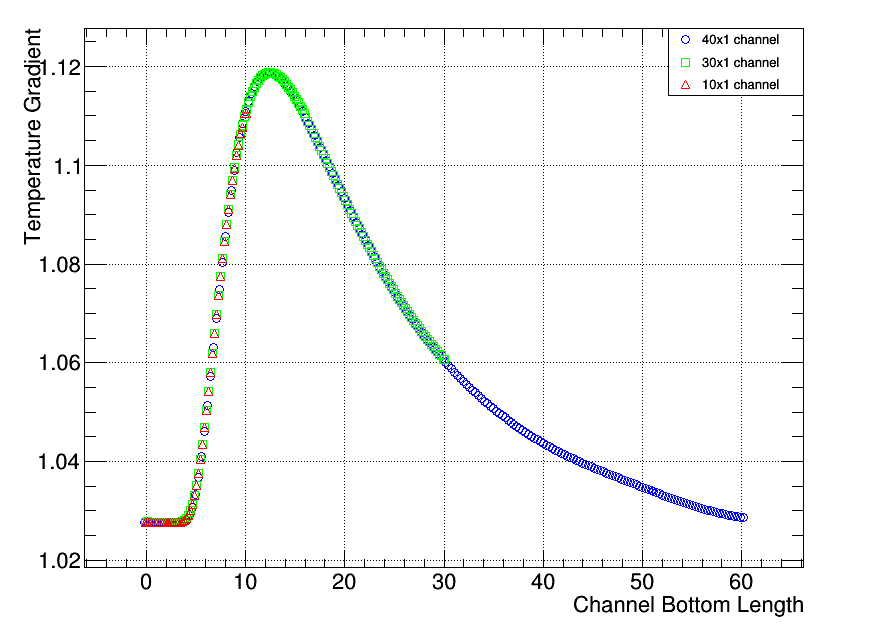
\includegraphics[width=0.75\linewidth]{chan}
\caption{Displays temperature gradient at bottom wall as a function of the channel length for varying channel lengths}
\label{chan1}
\end{figure}

\begin{table}[H]
\begin{center}
    \begin{tabular}{ | p{0.13\linewidth} | p{0.15\linewidth} |p{0.125\linewidth}|p{0.15\linewidth}|p{0.1\linewidth}|}
 \hline  
     \RaggedRight \textbf{Mesh Size}
    &\RaggedRight \textbf{${dT}/{dy}$}
    &\RaggedRight \textbf{Channel x}
    &\RaggedRight \textbf{Rel Error}
    &\RaggedRight \textbf{$GCI_{fine}$}
    \\ \hline  
           \RaggedRight 50 x 20
    &\RaggedRight 1.111794
      &\RaggedRight 12.25
       &\RaggedRight -
        &\RaggedRight -
    \\ \hline 
    		\RaggedRight 100 x 40
    &\RaggedRight 1.112606
    &\RaggedRight 12.30
     &\RaggedRight 8.121$*10^{-3}$
      &\RaggedRight -
    \\ \hline 
           \RaggedRight 200 x 80
    &\RaggedRight  1.114209 
    &\RaggedRight 12.20
    &\RaggedRight 1.603$*10^{-3}$
     &\RaggedRight 0.00184$\%$
    \\ \hline 
   
    \end{tabular}
\end{center} 
\caption{Gradient Solution for increasing mesh size using implicit method $\triangle t$ = 0.1}
\label{norm} 
\end{table}

\begin{figure}[H]
\centering
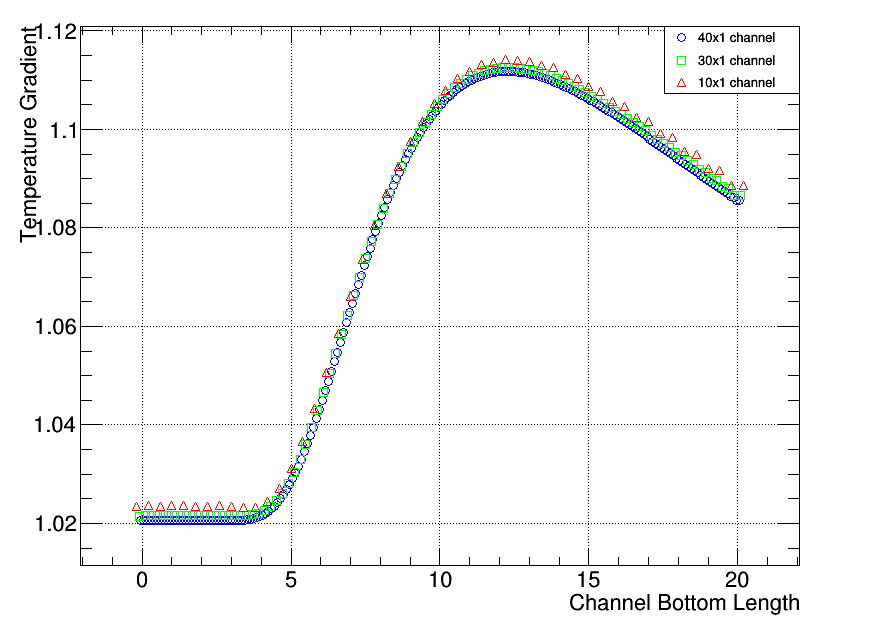
\includegraphics[width=0.75\linewidth]{chan2}
\caption{Displays the effect of mesh refinement on gradient solution}
\label{chan2}
\end{figure}

\section{Conclusion}
This project provides great insight into the internal algorithms used for calculating numerical solutions for time varying problems. The Energy Equation applied to a steady state channel provided a great platform for developing and testing the program. Having the analytic solution really help fine tune the program and helped given an idea on how accurate the solutions could be. Investigating the error and how it changes relative to boundaries and mesh sizes will provides insight on how the methods should be applied to bigger problems to minimize time and error. Stability analysis provided a great means for understanding the computational limits of the program in terms of speed. Numerical methods provide a great way of solving difficult problems and until new methods are discovered for finding exact solution will remain the main method for finding solutions to difficult problems. 





\newpage
\appendix
\section{Appendix} \label{App:Appendix}
\subsection{FinalProb.cpp}
\begin{lstlisting}
/*-------------------------------------------------------------------------------//
Main Program for finding solutions for energy equation. Employs a implicit euler
time advance with 2nd order centered flux scheme.


Jerin Roberts 2016
compiled using g++/gcc version 5.4.0 on Ubuntu 16.04.02 and are available for clone 
via the link provided: url{https://github.com/j16out/
//-------------------------------------------------------------------------------*/


#include <vector>
#include <iostream>
#include <cstdlib>
#include <fstream>
#include <string>
#include <vector>
#include <algorithm>
#include <sstream>
#include <math.h> 
#include "TApplication.h"
#include "vroot/root.hpp"
#include "numerical/numerical.hpp"

using namespace std;




int main(int argc, char **argv)
{
cdata mydata;

carray flow1;//my main array
carray flow2;
carray flow3;


//set array size or default used 162x162
set_array_size(flow1, 200, 80, 40.0, 1.0, 0);//array, xsize, ysize, dimension
set_array_size(flow2, 100, 40, 40.0, 1.0, 0);
set_array_size(flow3, 50, 20, 40.0, 1.0, 0);


set_zero(flow1);
set_zero(flow2);
set_zero(flow3);


//---------------------solve IE----------------------//
solve_array_IE(flow1, 14.5, 0.1);
solve_array_IE(flow2, 14.5, 0.1);
solve_array_IE(flow3, 14.5, 0.1);

//print_array(flow1);
double dx = 0.0;

find_max(flow1, dx);
get_discrete_Error(flow1, flow2, flow3);
//----------------------Draw Data---------------------//
if(1)//start root application
{
	TApplication theApp("App", &argc, argv);//no more than two subs  
	//draw_3Dgraph(flow1, flow2);
	find_maxvalues(flow1, flow2, flow3);
	theApp.Run();
}



//end
}

\end{lstlisting}
\subsection{numerical.hpp}
\begin{lstlisting}
#ifndef numerical_INCLUDED
#define numerical_INCLUDED


#include <vector>
#include <iostream>
#include <cstdlib>
#include <fstream>
#include <string>
#include <vector>
#include <algorithm>
#include <sstream>
#include <math.h> 
#include <iomanip>

using namespace std;

#define BIG 10000
#define maxx 202
#define maxy 82
#define PI 3.141592654

#define U0 3
#define T0 1
#define V0 1

#define RE 50
#define PR 0.7
#define EC 0.001



struct carray{
//arrays

double f1 [maxx][maxy];//second stage solution mesh
double T1 [maxx][maxy];//first stage and solution mesh
double v1 [maxx][maxy];//first stage and solution mesh
double u1 [maxx][maxy];
//array attributes
int sizex = maxx;
int sizey = maxy;
double DIMx = 0.0;
double DIMy = 0.0;
//scheme
int scheme = 0;
double ctime = 0;
};



struct cdata{
//data storage specific to array
vector<double> l2norm;
vector<double> l1norm;
vector<double> linfnorm;
vector<double> time1;
vector<double> time2;
};

struct crow{
//data for loaded row
double LHS [maxx][3];
double RHS [maxx];
};

struct ccol{
//data for loaded col
double LHS [maxy][3];
double RHS [maxy];
};

struct surr{
//surrounding cells
double Tim1_j = 0;
double Tip1_j = 0;
double Ti_j = 0; 
double Ti_jm1 = 0;
double Ti_jp1 = 0;

double uim1_j = 0;
double uip1_j = 0;
double ui_j = 0;
double ui_jm1 = 0;
double ui_jp1 = 0; 


double vim1_j = 0;
double vip1_j = 0;
double vi_j = 0; 
double vi_jm1 = 0;
double vi_jp1 = 0;
};


//--------------------Init Arrays-----------------------------------------//

void set_zero(carray & myarray);//zero entire array

void set_array_size(carray & myarray, int x, int y, double DIMx, double DIMy, int scheme);//set array size


//-------------------Boundary and Intial Conditions------------------------//

void set_ghostcells(carray & myarray);//set ghost cells

void set_intial_cond(carray & myarray);


//--------------------Solve Implicit Euler------------------------------------//

void solve_array_IE(carray & myarray, double tmax, double cfl);

void solve_LinSys(carray & myarray, double tstep, double & mdiff);

void load_row(carray & myarray, crow & myrow, int j, double tstep);

void load_col(carray & myarray, ccol & mycol, int i, double tstep);

void solve_thomas(crow & r, int iSize);

void solve_thomas(ccol & r, int iSize);


//--------------------Solve Explicit Euler------------------------------------//

void solve_array_EE(carray & myarray, double tmax, double cfl);

void time_advance_EE(carray & myarray, double tstep, double & mdiff);


//--------------------Flux calculation------------------------------------//

void compute_Flux(carray & myarray);

void get_nsurcells(carray & myarray, int i, int j, surr & mysurr);

double calc_newcell(carray & myarray, surr & s1);



//-----------------------Error calc related functions---------------------------//

double get_l2norm(carray & myarray, carray myarray2);//get estimated vale for l2 norm between arrays

double get_l1normD(carray & myarray, carray myarray2);

void set_analytic(carray & myarray, carray & numarray);//set analytic solution to a mesh

void get_discrete_Error(carray ray1, carray ray2, carray ray3);

//-----------------------Print related functions-------------------------------//

void print_array(carray & myarray);//print array in terminal

void print_arrayu(carray & myarray);

void print_row(crow & myrow, carray & myarray);

void print_col(ccol & mycol, carray & myarray);

void find_max(carray & myarray, double & dx);

#endif

\end{lstlisting}
\subsection{numerical.cpp}
\begin{lstlisting}
#include "numerical.hpp"





//**************************************************************************//
//---------------------------Setting Array----------------------------------//
//**************************************************************************//


//----------set array size (working area excluding ghost)---------------//

void set_array_size(carray & myarray, int x, int y, double DIMx, double DIMy, int scheme)
{
	if(x <= maxx && y <= maxy)
	{
	myarray.sizex = x+2;
	myarray.sizey = y+2;
	myarray.DIMx = DIMx/(x);
	myarray.DIMy = DIMy/(y);
	myarray.scheme = scheme;
	}
	else
	cout << "Array size to big, setting to default 100" << "\n";

}




//--------------------------zero array----------------------------//

void set_zero(carray & myarray)
{
	for(int j = 0; j < myarray.sizey; ++j)
	{
		for(int i = 0; i < myarray.sizex; ++i)
		{
		myarray.T1[i][j] = 0;//set everything to zero
        myarray.f1[i][j] = 0;
        myarray.v1[i][j] = 0;
        myarray.u1[i][j] = 0;

		}
	}
}


//--------------------------set ghost cells for Energy----------------------------//


void set_ghostcells(carray & myarray)
{
double DIMx = myarray.DIMx;
double DIMy = myarray.DIMy;
double dx = 0.0;
double dy = 0.0;
    //set ghost cells top/bottom
	for(int i = 0; i < myarray.sizex; ++i)
	{
	dx = (i-0.5)*DIMx;
	myarray.T1[i][0] = 3.0*(0.0) - (5.0/2.0)*myarray.T1[i][1] + (1.0/2.0)*myarray.T1[i][2];
	
	    if( dx <= 3.0 && dx >= 1.0) 
	    {
	    myarray.T1[i][myarray.sizey-1] =3.0*(2-cos(PI*(dx-1)))- (5.0/2.0)*myarray.T1[i][myarray.sizey-2] + (1.0/2.0)*myarray.T1[i][myarray.sizey-3];
	    }
	    else
	    {
	    myarray.T1[i][myarray.sizey-1] =3.0*(1.0)- (5.0/2.0)*myarray.T1[i][myarray.sizey-2] + (1.0/2.0)*myarray.T1[i][myarray.sizey-3];
	    }
	}	
	
    //set ghost cells inflow/outflow	
	for(int j = 0; j < myarray.sizey; ++j)
	{ 
    dy = (j-0.5)*DIMy;
    
	myarray.T1[0][j] = 2.0*( dy+((3.0/4.0)*PR*EC*(pow(U0,2))*(1.0-pow((1.0-2.0*dy),4))) ) - myarray.T1[1][j];
	
	
	myarray.T1[myarray.sizex-1][j] = myarray.T1[myarray.sizex-2][j];

	}
}

//--------------------------set intial condition---------------------------------//

void set_intial_cond(carray & myarray)
{
double DIMx = myarray.DIMx;
double DIMy = myarray.DIMy;
double dx = 0.0;
double dy = 0.0;

for(int j = 0; j < myarray.sizey; ++j)
{

    for(int i = 0; i < myarray.sizex; ++i)
    {
    dy = (j-0.5)*DIMy;
    
    myarray.T1[i][j] = dy;
    myarray.u1[i][j] = 6.0*U0*dy*(1.0-dy);
    myarray.v1[i][j] = 0;
    //printf("f: %f  dx: %f\n", f, dx);
    }

}
}

//**************************************************************************//
//-----------------------------IE Array Solving-----------------------------//
//**************************************************************************//

void solve_array_IE(carray & myarray, double tmax, double cfl)
{

//double tstep = (cfl*(myarray.DIMx))/2.0;
double tstep = cfl;
double ctime = 0.0;

set_intial_cond(myarray);
set_ghostcells(myarray);

printf("\n\nRunning size: %d time step: %f\n",myarray.sizex,tstep);


int n = 0;
int nt = 10;
double mdiff = 0;

while(ctime < tmax-tstep)
{

//implicit time advance
ctime = ctime+tstep;
compute_Flux(myarray);
solve_LinSys(myarray, tstep, mdiff);
set_ghostcells(myarray);

//print_array(myarray);


if(n >= nt)//status
{
printf("Run: %d time: %f diff %f\n",n,ctime, mdiff);
nt = 10+n;
} 
if(mdiff<0.000001)
break; 

++n;
}

myarray.ctime = ctime;

printf("Solved numeric at %f time with tstep %f\n",ctime, tstep);

}

//-------------------------------LHS approx factor----------------------//

void solve_LinSys(carray & myarray, double tstep, double & mdiff)
{
mdiff = -1.0;
//--linear system num 1---//
crow myrow;
//print_array(myarray);
//print_arrayu(myarray);

for(int j = 0; j < myarray.sizey; ++j)
{

load_row(myarray, myrow, j, tstep);
solve_thomas(myrow, myarray.sizex);

    for(int i = 0; i < myarray.sizex; ++i)
    {
    myarray.f1[i][j] = myrow.RHS[i];
    }
}

//print_array(myarray);
//print_arrayu(myarray);

//--linear system num 2---//
ccol mycol;
for(int i = 0; i < myarray.sizex; ++i)
{
load_col(myarray, mycol, i, tstep);
solve_thomas(mycol, myarray.sizey);

    for(int j = 0; j < myarray.sizey; ++j)
    {
    double temp = mycol.RHS[j];
    if(abs(temp) > mdiff)
    mdiff = abs(temp);
    myarray.f1[i][j] = temp;
    myarray.T1[i][j] = temp + myarray.T1[i][j];
    }
}
//print_arrayu(myarray);
}



//--------------------------Load row for Thomson---------------------------//

void load_row(carray & myarray, crow & myrow, int j, double tstep)
{
double chx = myarray.DIMx;
for(int i = 0; i < myarray.sizex; ++i)
{

double alpha = tstep/(RE*PR*pow(chx,2.0));
double beta = (myarray.u1[i][j]*tstep)/(2.0*chx);
if(i == 0)
{
myrow.LHS[i][0] = 0.0;
myrow.LHS[i][1] = 1.0;
myrow.LHS[i][2] = 1.0;
}
else if(i == myarray.sizex-1)
{
myrow.LHS[i][0] =  -1.0;
myrow.LHS[i][1] =  1.0;
myrow.LHS[i][2] =  0.0;
}
else
{
myrow.LHS[i][0] = (-alpha - beta);
myrow.LHS[i][1] = (1.0 + 2.0*alpha);
myrow.LHS[i][2] = (-alpha + beta);
}
//load the flux

myrow.RHS[i] = tstep * myarray.f1[i][j];
}

}



//--------------------------Load column for Thomson---------------------------//

void load_col(carray & myarray, ccol & mycol, int i, double tstep)
{
double chy = myarray.DIMy;
for(int j = 0; j < myarray.sizey; ++j)
{
double alpha = tstep/(RE*PR*pow(chy,2));
double beta = (myarray.v1[i][j]*tstep)/(2.0*chy);


if(j == 0)
{
mycol.LHS[j][0] =  0.0;
mycol.LHS[j][1] =  1.0;
mycol.LHS[j][2] =  1.0;
}
else if(j == myarray.sizey-1)
{
mycol.LHS[j][0] =  1.0;
mycol.LHS[j][1] =  1.0;
mycol.LHS[j][2] =  0.0;
}
else
{
mycol.LHS[j][0] = (-alpha - beta);
mycol.LHS[j][1] = (1.0 + 2.0*alpha);
mycol.LHS[j][2] = (-alpha + beta);
}
//load the solution from first linsys solve
mycol.RHS[j] = myarray.f1[i][j]; 
}
mycol.RHS[0] = 0.0; 
mycol.RHS[myarray.sizey] = 0.0; 

}


//------------------------------Thomas solving----------------------------------//


void solve_thomas(crow & r, int iSize)
{
  int i;
  /* This next line actually has no effect, but it -does- make clear that
     the values in those locations have no impact. */
  r.LHS[0][0] = r.LHS[iSize-1][2] = 0;
  /* Forward elimination */
  for (i = 0; i < iSize-1; i++) {
    r.LHS[i][2] /= r.LHS[i][1];
    r.RHS[i] /= r.LHS[i][1];
    r.LHS[i+1][1] -= r.LHS[i][2]*r.LHS[i+1][0];
    r.RHS[i+1] -= r.LHS[i+1][0]*r.RHS[i];
  }
  /* Last line of elimination */
  r.RHS[iSize-1] /= r.LHS[iSize-1][1];

  /* Back-substitution */
  for (i = iSize-2; i >= 0; i--) {
    r.RHS[i] -= r.RHS[i+1]*r.LHS[i][2];
  }
  
}

void solve_thomas(ccol & r, int iSize)
{
  int i;
  /* This next line actually has no effect, but it -does- make clear that
     the values in those locations have no impact. */
  r.LHS[0][0] = r.LHS[iSize-1][2] = 0;
  /* Forward elimination */
  for (i = 0; i < iSize-1; i++) {
    r.LHS[i][2] /= r.LHS[i][1];
    r.RHS[i] /= r.LHS[i][1];
    r.LHS[i+1][1] -= r.LHS[i][2]*r.LHS[i+1][0];
    r.RHS[i+1] -= r.LHS[i+1][0]*r.RHS[i];
  }
  /* Last line of elimination */
  r.RHS[iSize-1] /= r.LHS[iSize-1][1];

  /* Back-substitution */
  for (i = iSize-2; i >= 0; i--) {
    r.RHS[i] -= r.RHS[i+1]*r.LHS[i][2];
  }
  
}

//**************************************************************************//
//-----------------------------EE Array Solving-----------------------------//
//**************************************************************************//

void solve_array_EE(carray & myarray, double tmax, double cfl)
{
double tstep = (cfl*(myarray.DIMx))/2.0;
double ctime = 0.0;
double mdiff = 0.0;
set_intial_cond(myarray);
set_ghostcells(myarray);

printf("\n\nRunning size: %d time step: %f\n",myarray.sizex,tstep);

int n = 0;
int nt = 10;

while(ctime < tmax-tstep)
{
  
ctime = ctime+tstep;
compute_Flux(myarray);
time_advance_EE(myarray, tstep, mdiff);

set_ghostcells(myarray);


if(n >= nt)//status
{
printf("Run: %d time: %f diff %f\n",n,ctime, mdiff);
nt = 10+n;
}
if(mdiff<0.000001)
break; 

++n;
}

myarray.ctime = ctime;
printf("Solved numeric at %f time with tstep %f\n",ctime, tstep);
}

//------------------------------EE time advance----------------------------//

void time_advance_EE(carray & myarray, double tstep, double & mdiff)
{
mdiff = -1.0;
for(int j = 1; j < myarray.sizey-1; ++j)
{
    for(int i = 1; i < myarray.sizex-1; ++i)
    {  
    double temp = tstep*(myarray.f1[i][j]); 
    if(abs(temp)> mdiff)
    mdiff = abs(temp);
       
    myarray.T1[i][j] = myarray.T1[i][j] + temp;
    }
}
}


//**************************************************************************//
//---------------------------Compute Flux-----------------------------------//
//**************************************************************************//


void compute_Flux(carray & myarray)
{
surr mysurr;

for(int j = 1; j < myarray.sizey-1; ++j)
{
    for(int i = 1; i < myarray.sizex-1; ++i)
    {
    //----get surrounding cells and compute new cell----//
    get_nsurcells(myarray, i, j, mysurr);
    //-----update current cell----//
    double newcell = calc_newcell(myarray, mysurr);    
    myarray.f1[i][j] = newcell;   
    }

}
}

//--------------------------get surrounding cells-----------------------//

void get_nsurcells(carray & myarray, int i, int j, surr & mysurr)
{

mysurr.Tim1_j = myarray.T1[i-1][j];
mysurr.Tip1_j = myarray.T1[i+1][j];
mysurr.Ti_j = myarray.T1[i][j]; 
mysurr.Ti_jm1 = myarray.T1[i][j-1];
mysurr.Ti_jp1 = myarray.T1[i][j+1];

mysurr.uim1_j = myarray.u1[i-1][j];
mysurr.uip1_j = myarray.u1[i+1][j];
mysurr.ui_jm1 = myarray.u1[i][j-1];
mysurr.ui_jp1 = myarray.u1[i][j+1];
 

mysurr.vi_jm1 = myarray.v1[i][j-1];
mysurr.vi_jp1 = myarray.v1[i][j+1];
mysurr.vim1_j = myarray.v1[i-1][j];
mysurr.vip1_j = myarray.v1[i+1][j];
}


//-----------------------calculate flux for new cell--------------------//

double calc_newcell(carray & myarray, surr & s1)
{
double chx = myarray.DIMx;
double chy = myarray.DIMy;
//double chy = DIM1;

double a = (s1.uip1_j * s1.Tip1_j  -  s1.uim1_j * s1.Tim1_j)/(2.0);
double b = (s1.Tip1_j  - 2.0*s1.Ti_j + s1.Tim1_j)/(chx*(RE*PR));
double c = (s1.vi_jp1 * s1.Ti_jp1  -  s1.vi_jm1 * s1.Ti_jm1)/(2.0);
double d = (s1.Ti_jp1  - 2.0*s1.Ti_j + s1.Ti_jm1)/(chy*(RE*PR));

double e = (2.0*pow((s1.uip1_j-s1.uim1_j)/(2.0*chx),2)+2.0*pow((s1.vi_jp1-s1.vi_jm1)/(2.0*chy),2));
double f = pow(((s1.vip1_j-s1.vim1_j)/(2.0*chx))+((s1.ui_jp1-s1.ui_jm1)/(2.0*chy)), 2);
double source = (EC/RE)*(e+f);

double newcell = 1.0*((-1.0/chx)*(a-b)   +   (-1.0/chy)*(c-d))   +   source;
return newcell;
}



//**************************************************************************//
//---------------------------Error Checking---------------------------------//
//**************************************************************************//
//--------------------------Get descrete error----------------------------//

void get_discrete_Error(carray ray1, carray ray2, carray ray3)
{
//Calculating error as described in paper "procedure for estimation and reporting of uncertainty due to discretization in CFD applications"//

printf("\nCalculating Error...\n");

double h1 = ray1.DIMx;
double h2 = ray2.DIMx;
double h3 = ray3.DIMx;

/*
double sol1 = ray1.T1[40][20];
double sol2 = ray2.T1[20][10];
double sol3 = ray3.T1[10][5];
*/
double sol1 = 1.114209;
double sol2 = 1.112606;
double sol3 = 1.111794;




printf("h1: %f \nh2: %f \nh3: %f, \nsol1: %f \nsol2: %f \nsol3: %f\n",h1, h2, h3, sol1, sol2, sol3);

double r21 = h2/h1;
double r32 = h3/h2;

printf("\nr32: %f \nr21: %f\n",r32, r21);

double e32 = sol3-sol2;
double e21 = sol2-sol1;

double s = (e32/e21);
if(s >= 0)
s = 1;
else
s = -1;

double p_n = 0;
double p = (1/log(r21))*(abs(log(abs(e32/e21))+0));

printf("intial guess: %f \n", p);

double diff = 1;

	while(diff > 0.0000001)
	{

	double p_n = (1/log(r21))*(abs(log(abs(e32/e21))+log((pow(r21,p)-s)/(pow(r32,p)-s)) ));
	diff = abs(p_n -p);
	//printf("p_n: %f p: %f diff: %f\n",p_n, p, diff);

	p = p_n;
	}
 
//
double sol_ext21 = (pow(r21, p)*sol1-sol2)/(pow(r21,p)-1.0);
double sol_ext32 = (pow(r32, p)*sol2-sol3)/(pow(r32,p)-1.0);

printf("order: %f \nphi_ext21: %f \nphi_ext32 %f\n",p, sol_ext21, sol_ext32);

double ea21 = abs((sol1-sol2)/sol1);

double e_ext21 = abs((sol_ext21-sol1)/sol_ext21);

double GCI_21 = (1.25*ea21)/(pow(r21,p)-1.0);


printf("ea21: %f  \ne_ext21: %f  \nGC121 %f \n", ea21, e_ext21, GCI_21);

}
//-------------------------------------l2norm--------------------------//

double get_l2norm(carray & myarray, carray myarray2)
{
double l2sum =0;

double sx = myarray.sizex-2;
double sy = myarray.sizey-2;

for(int j = 1; j < myarray.sizey-1; ++j)
{	
	for(int i = 1; i < myarray.sizex-1; ++i)
	{
	double P = myarray.f1[i][j];
	double T = myarray2.f1[i][j];
	l2sum =  l2sum + pow((P-T),2);

	}


}

double l2 = sqrt(l2sum/(sx*sy));
cout << setprecision(8) << fixed << "L2 norm: " << l2 << "\n";
return l2;
}

//-------------------------------------l2norm between diff--------------------------//

double get_l1normD(carray & myarray, carray myarray2)
{
double l2sum =0;

double sx = myarray.sizex-2;
double sy = myarray.sizey-2;

for(int j = 1; j < myarray.sizey-1; ++j)
{	
	for(int i = 1; i < myarray.sizex-1; ++i)
	{
	double P = myarray.f1[i][j];
	double T = myarray2.f1[i*2][j*2];
	l2sum =  l2sum + abs(P-T);

	}


}

double l2 = l2sum/(sx*sy);
cout << setprecision(9) << fixed << "L1 norm: " << l2 << "\n";
return l2;
}

//----------------------------Set a Analytical Solution------------------------------//
void set_analytic(carray & myarray, carray & numarray)
{
double DIMx = myarray.DIMx;
double DIMy = myarray.DIMy;
double ctime = numarray.ctime;
for(int j = 1; j < myarray.sizey-1; ++j)
{

	for(int i = 1; i < myarray.sizex-1; ++i)
	{
	double dx = (i-0.5)*DIMx;
	double dy = (j-0.5)*DIMy;
	
	double a = U0*T0*PI*cos(2.0*PI*dx)*dy*sin(PI*dy);
	double b = V0*T0*PI*dx*cos(PI*dx)*cos(2.0*PI*dy);
	double c = (2.0*T0*pow(PI,2)*cos(PI*dx)*sin(PI*dy))/(RE*PR);
	
	double d = pow((U0*sin(PI*dx)+V0*cos(PI*dy)), 2);
	double source = (EC/RE)*((2.0*pow((U0*PI*cos(PI*dx)*dy),2)+(2.0*pow((V0*PI*sin(PI*dy)*dx),2)))+d);
	myarray.f1[i][j] =  a + b + c + source;
	
	}

}

printf("setting analytic at %f time\n",ctime);
}

//**************************************************************************//
//---------------------------Print Functions--------------------------------//
//**************************************************************************//





//--------------------------zero array----------------------------//

void find_max(carray & myarray, double & dx)
{double temp;
 double mdif = -1000.0;
 double DIMx = myarray.DIMx;
	for(int j = 1; j < 10; ++j)
	{
		for(int i = 0; i < myarray.sizex; ++i)
		{
		temp = myarray.T1[i][j];//set everything to zero
            if(temp > mdif)
            {
            mdif = temp;
            dx = (i-0.5)*DIMx;
            
            }

		}
		printf("dx: %f\n", dx);
	}
	
}
//--------------------------Print array in terminal----------------------------//

void print_array(carray & myarray)
{
cout << "Solution:\n       |";
for(int i = 0; i < myarray.sizex; ++i)
		{
		if(i < 10)
		cout << "   i: " << i <<"|";
		if(i > 9)
		cout << "   i:" << i <<"|";
        }
cout << "\n";
	for(int j = 0; j < myarray.sizey; ++j)
	{
	if(j > 9)
	cout << "\nj:" << j << "|  |";
	if(j < 10)	
	cout << "\nj: " << j << "|  |";
		for(int i = 0; i < myarray.sizex; ++i)
		{
		if(myarray.T1[i][j] >= 0)
		cout << setprecision(5) << fixed << myarray.T1[i][j] <<"|";
		if(myarray.T1[i][j] < 0)
		cout << setprecision(4) << fixed << myarray.T1[i][j] <<"|";
		}
	
	}
cout << "\n\n";
}

//--------------------------Print u array in terminal----------------------------//

void print_arrayu(carray & myarray)
{

cout << "Flux:\n       |";
for(int i = 0; i < myarray.sizex; ++i)
		{
		if(i < 10)
		cout << "   i: " << i <<"|";
		if(i > 9)
		cout << "   i:" << i <<"|";
        }
cout << "\n";
	for(int j = 0; j < myarray.sizey; ++j)
	{
	if(j > 9)
	cout << "\nj:" << j << "|  |";
	if(j < 10)	
	cout << "\nj: " << j << "|  |";
		for(int i = 0; i < myarray.sizex; ++i)
		{
		if(myarray.f1[i][j] >= 0)
		cout << setprecision(5) << fixed << myarray.f1[i][j] <<"|";
		if(myarray.f1[i][j] < 0)
		cout << setprecision(4) << fixed << myarray.f1[i][j] <<"|";
		}
	
	}
cout << "\n\n";
}


//-------------------------------print row------------------------------------//

void print_row(crow & myrow, carray & myarray)
{
cout << "\nprint rows\n";
for(int i = 0; i < myarray.sizex; ++i)
{
cout << "|" << myrow.LHS[i][0] << "|" << myrow.LHS[i][1] << "|" << myrow.LHS[i][2] << "|   |" << myrow.RHS[i] << "|\n";

}

}



void print_col(ccol & mycol, carray & myarray)
{
cout << "\nprint rows\n";
for(int i = 0; i < myarray.sizey; ++i)
{
cout << "|" << mycol.LHS[i][0] << "|" << mycol.LHS[i][1] << "|" << mycol.LHS[i][2] << "|   |" << mycol.RHS[i] << "|\n";

}

}

/*
void set_ghostcells(carray & myarray)
{
double DIMx = myarray.DIMx;
double DIMy = myarray.DIMy;
double dx = 0.0;
double dy = 0.0;
    //set ghost cells top/bottom
	for(int i = 0; i < myarray.sizex; ++i)
	{
	myarray.T1[i][0] = 2.0*(0.0) - myarray.T1[i][1];
	myarray.T1[i][myarray.sizey-1] =2.0*(1.0)-myarray.T1[i][myarray.sizey-2];
	}	
	
    //set ghost cells inflow/outflow	
	for(int j = 0; j < myarray.sizey; ++j)
	{ 
    dy = (j-0.5)*DIMy;
    
	myarray.T1[0][j] = 2.0*( dy+((3.0/4.0)*PR*EC*(pow(U0,2))*(1.0-pow((1.0-2.0*dy),4))) ) - myarray.T1[1][j];
	
	
	myarray.T1[myarray.sizex-1][j] = myarray.T1[myarray.sizex-2][j];

	}
}
*/



\end{lstlisting}

\begin{thebibliography}{99} % Beamer does not support BibTeX so references must be inserted manually as below
\bibitem[Celik, 2006]{p0}Ismail B. Celik1, Urmila Ghia, Patrick J.Roache and Christopher J. Freitas
\newblock "Procedure for Esitmation and Reporting Uncertainty Due to Discretization in CFD apllications",  West Virginia University, Morgantown WV, USA

\end{thebibliography}


%%% End document
\end{document}